\documentclass[aps,prb,twocolumn,superscriptaddress,floatfix]{revtex4-2}
\usepackage{graphicx,amsmath,amssymb,bm,xcolor}
\usepackage[colorlinks=true,linkcolor=blue,citecolor=blue,urlcolor=blue]{hyperref}
\newtheorem{theorem}{Theorem}
\newcommand{\eps}{\varepsilon}
\begin{document}

\title{Quantum selection of eightfold rhombus tilings:\\ faceting at zero field and a charge-budget magnetization staircase}

\author{Changyeon Won}
\affiliation{Department of Physics, Kyung Hee University, Seoul 02447, Republic of Korea}

\date{\today}

\begin{abstract}
All eightfold (Ammann--Beenker type) rhombus tilings have the same classical Heisenberg energy, so the exchange graph itself is chosen by quantum fluctuations. We study the spin-$1/2$ antiferromagnet on these tilings with exact combinatorial results, linear spin-wave theory, and sign-free quantum Monte Carlo. Three results stand out. (i) At zero field the quasiperiodic tiling is unstable. The ground state at fixed composition is macroscopically faceted into domains whose exchange graph is exactly the square lattice. Such domains exist only when the tile types split the ribbon families into two cyclic intervals, folds between them cost nothing, and one topologically fixed defect quintet remains per period. (ii) In a field, exact angle and Euler identities express the Lieb magnetization through the mean curvature charge of one sublattice, $m=\kappa_B/(4+\kappa_B)$. Every plateau bound is the saturation of a linear budget in the square fraction $c$: $m\le(1-c)/2$, $m\le c/3$, and $m\le 1/5$. The thermodynamic limit reduces to a linear program in two conserved resources. We search all winding sectors of periodic tilings with up to $24$ tiles per cell ($5761$ sectors, $3.2\times10^5$ tilings) and simulate every phase on the ground-state path directly. Magnetization sets in at $h\simeq0.07J$ through isolated sixfold hubs. A plateau at exactly the composition-independent bound $m=1/5$ follows, carried by hub-free crystals, and the curve ends with a jump into dice-lattice domains at $h\simeq0.27J$. Both features are present in at least $97\%$ of resampled energy sets. Between these, the selected crystals are rational approximants of the irrational square-to-rhombus ratio $1/\sqrt2$. The plateau values there change with cell size, and we argue that they do not converge. (iii) The ratio of exact to harmonic phase energies varies from $0.86$ to $1.29$ and grows with the carrier charge density. The first magnon-interaction (Hartree) correction, which measures how suppressed and enhanced bond fluctuations compensate, predicts it for $35$ phases whose ratios were recorded before simulation, with an rms error of $0.04$ and a slight systematic underestimate for hub-free crystals.
\end{abstract}

\maketitle

%=====================================================================
\section{Introduction}
%=====================================================================

When a classical ground state is degenerate, fluctuations usually decide which state is realized~\cite{Villain1980,Henley1989,Henley2006}. The degeneracy is almost always among spin configurations on a fixed lattice. A stronger form of degeneracy appears when the lattice itself can change. If a whole family of exchange graphs has the same classical energy, the zero-point energy of the spins selects the graph. Rhombus tilings realize this situation naturally. A tiling is a graph, local tile flips change the graph, and in many cases the graph is bipartite, so that the Heisenberg antiferromagnet obeys Lieb's theorem~\cite{LiebMattis1962,Lieb1989} and can be simulated without a sign problem~\cite{Sandvik1999,Syljuasen2002,Sandvik2010}. Classically, the same tilings are random-tiling and height models~\cite{BloteHilhorst1982,Henley1991,KOS2006}, and local tile flips are the kinetic terms of quantum dimer models~\cite{Rokhsar1988,Moessner2001,Moessner2001b}.

Quasicrystalline antiferromagnets have been studied on fixed tilings, notably the Penrose and Ammann--Beenker tilings, where the inhomogeneous coordination produces a rich pattern of local staggered moments~\cite{Wessel2003,Jagannathan2004,Jagannathan2006,Szallas2008,Jagannathan2012}. Phason disorder of such tilings was found to lower the antiferromagnetic ground-state energy~\cite{Szallas2009}, and geometric fluctuations act on the spins through Casimir-type forces~\cite{Jagannathan2013}; similar inhomogeneous ground states arise on percolating clusters~\cite{WangSandvik2006}. Here we ask the complementary question. Which tiling does the quantum antiferromagnet prefer, and how does a magnetic field change the answer? We consider eightfold rhombus tilings~\cite{Beenker1982,Ammann1992} built from squares and $45^\circ$ rhombi. Compared with threefold (lozenge) tilings, they offer four ribbon families instead of three, two tile shapes, a free composition $c$ (the square fraction; $c=\sqrt2-1$ for Ammann--Beenker), and a genuinely quasiperiodic candidate whose stability can be tested. A companion study treats the threefold case, where the tilings interpolate between the dice lattice, whose flat bands and Aharonov--Bohm cages make it a standard bipartite model~\cite{Sutherland1986,Vidal1998}, and the honeycomb antiferromagnet. It finds a staircase of hub-free crystals bounded by the same kind of counting~\cite{Yoo2026}. The two problems share the Lieb-sector QMC procedure, the convexity arguments, and the hub-free bound; here we concentrate on what is new with four families and two tile shapes.

Our central finding is that most of the physics is fixed by counting rather than by energetics. Exact identities fix the magnetization in terms of curvature charges of the exchange graph. A classification theorem fixes which domains are free of defects, and Gauss--Bonnet fixes how many defects must remain. Linear budgets fix the plateau values. Energetics then decides only which of the allowed structures is realized. Where no budget line passes through the sample composition, the choice falls on rational approximants of an irrational composition, and the finite-cell staircase need not converge. We compute it with linear spin-wave theory (LSWT)~\cite{Anderson1952} and calibrate it phase by phase with quantum Monte Carlo (QMC). We find, unexpectedly, that the QMC correction is not a uniform renormalization. It depends on the density of curvature charges in a way that the first magnon-interaction correction~\cite{Oguchi1960} predicts quantitatively.

The paper is organized as follows. Section~\ref{sec:model} introduces the model and the exact magnetization identities. Section~\ref{sec:zero} proves that the zero-field ground state is faceted and identifies the topological defects. Section~\ref{sec:field} derives the budget lines, the ribbon carriers, the magnetization staircase, and the balance of exchange and Zeeman energy along it. Section~\ref{sec:hartree} explains the phase dependence of quantum corrections and presents the blind test. Section~\ref{sec:disc} discusses what is model independent and what can be tested.

%=====================================================================
\section{Model and exact identities}\label{sec:model}
%=====================================================================

\subsection{Tilings, bipartiteness, and classical degeneracy}

The edges of an eightfold rhombus tiling are the vectors $\pm\mathbf v_j$ with $\mathbf v_j=(\cos\frac{\pi(j-1)}4,\sin\frac{\pi(j-1)}4)$, $j=1,\dots,4$ [Fig.~\ref{fig:tiles}(a)]. Each vertex lifts to a point $\mathbf n\in\mathbb Z^4$~\cite{deBruijn1981}. A tile spanned by $\mathbf v_1,\mathbf v_3$ or $\mathbf v_2,\mathbf v_4$ is a square, and the other four pairs give $45^\circ$ rhombi. We place spins $S=1/2$ on the vertices,
\begin{equation}
H=J\sum_{\langle ij\rangle}\mathbf S_i\cdot\mathbf S_j-h\sum_i S_i^z,\qquad J>0 .
\label{eq:H}
\end{equation}
Every edge changes $\sum_a n_a$ by one, so the parity of the lifted coordinate sum defines a bipartition into sublattices $A$ and $B$ for every tiling. All faces are quadrilaterals, and Euler's relation on a torus gives exactly $2N$ bonds for $N$ sites. The classical N\'eel energy $-2JS^2N$ is therefore the same for all tilings, and only quantum fluctuations distinguish them. A tile flip moves a threefold vertex across its hexagon, $\mathbf n\to\mathbf n\pm\mathbf e_a\pm\mathbf e_b\pm\mathbf e_c$. It changes the parity of one site and hence $N_A-N_B$ by $\pm2$.

\begin{figure*}[t]
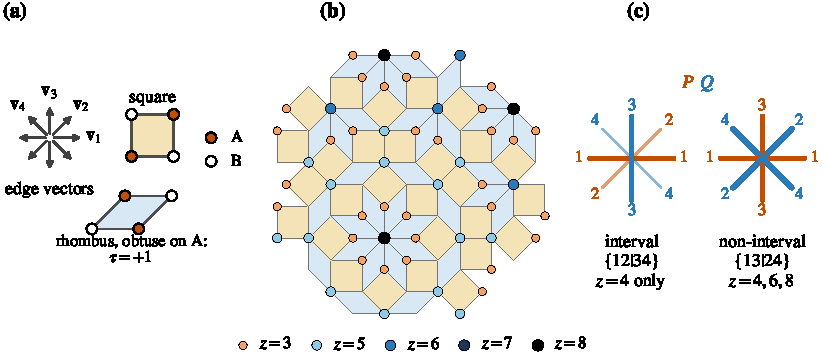
\includegraphics[width=\textwidth]{figs/fig1.pdf}
\caption{(a)~Edge vectors and tiles. Sublattices alternate around every tile. A rhombus has $\tau=+1$ if its obtuse corners lie on $A$. (b)~A patch of the Ammann--Beenker tiling. Squares and rhombi are shaded, and vertices with $z\neq4$ are marked. (c)~Edge directions around a vertex, labeled by a bipartition $P|Q$ of the ribbon families. Consecutive edges must alternate between $P$ and $Q$. For an interval split such as $\{12|34\}$ the eight directions form four blocks and force $z=4$. The non-interval split $\{13|24\}$ alternates at every step and allows $z=4,6,8$; the eightfold hubs of the quasicrystal are of this type.}
\label{fig:tiles}
\end{figure*}

\subsection{Magnetization as rhombus polarization}

By Lieb's theorem the ground state at $h=0$ has total spin $S_{\rm tot}=S|N_A-N_B|$~\cite{LiebMattis1962,Lieb1989}. Such ferrimagnets are stable and have no Anderson tower of states~\cite{Rademaker2020}. Summing the tile angles at every vertex ($360^\circ$) over each sublattice gives
\begin{align}
360N_A&=180S_\square+270R_A+90R_B,\nonumber\\
360N_B&=180S_\square+90R_A+270R_B ,
\end{align}
where $S_\square$ is the number of squares and $R_A$ ($R_B$) is the number of rhombi whose obtuse corners lie on $A$ ($B$). Subtracting the two equations gives
\begin{equation}
M\equiv N_A-N_B=\frac12\sum_{\rm rhombi}\tau_t,\qquad \tau_t=\pm1 .
\label{eq:tau}
\end{equation}
Squares carry no moment. The Lieb moment is the polarization of an Ising variable attached to each rhombus [Fig.~\ref{fig:tiles}(a)]. With $c=S_\square/N$ and $R/N=1-c$ this gives the first bound,
\begin{equation}
m\equiv M/N\le(1-c)/2 .
\label{eq:mmax}
\end{equation}

\subsection{Magnetization as mean curvature charge}

In the graph metric, where every tile is a unit square, a vertex of coordination $z$ carries curvature charge $q=4-z$. Every bond has one end on each sublattice, so $\sum_A z=\sum_B z=2N$. Define the mean charges $\kappa_B=\sum_B(z-4)/N_B$ on the minority sublattice and $\kappa_A=\sum_A(4-z)/N_A$ on the majority sublattice. Then
\begin{equation}
m=\frac{\kappa_B}{4+\kappa_B}=\frac{\kappa_A}{4-\kappa_A} .
\label{eq:kappa}
\end{equation}
The magnetization is fixed entirely by the mean curvature charge of one sublattice. Since $z\ge3$, $\kappa_A\le1$ and $m\le1/3$, the dice-lattice value. If the minority sublattice carries no net charge beyond one per site, $\kappa_B\le1$, then $m\le1/5$. These bounds hold for any tiling, any spin length, and any interaction that depends only on the graph.

%=====================================================================
\section{Zero field: quantum faceting}\label{sec:zero}
%=====================================================================

\subsection{Which domains are free of defects}

Around a vertex the edges, ordered by angle, enclose tiles, and consecutive edges are separated by $45^\circ$, $90^\circ$, or $135^\circ$. Suppose the tile types present in a region define a bipartite graph on the four ribbon families with parts $P$ and $Q$. Then consecutive edges must alternate between $P$ and $Q$, and a gap can never exceed $135^\circ$.

\begin{theorem}[Interval classification]
All interior vertices of a region have $z=4$ if and only if its tile-type graph is bipartite with both parts cyclic intervals of the family order $1,2,3,4$. For $n$ families there are $\binom n2$ such classes. For $n=4$ these are the pair splits $A=\{12|34\}$ and $B=\{14|23\}$ and four star splits.
\end{theorem}

For an interval split the eight directions fall into four alternating blocks, and a gap of at most $135^\circ$ cannot skip a block, so $z=4$ [Fig.~\ref{fig:tiles}(c)]. The non-interval split $\{13|24\}$ alternates at every $45^\circ$ and allows $z=4,6,8$. This is exactly the eightfold star of the Ammann--Beenker tiling. Combining a triangle lemma (three pairwise-crossing ribbons enclose a threefold cell) with the monotonicity of ribbons shows that extended uniform domains are of class $A$ or $B$ only (Appendix~\ref{app:proofs}). The eightfold rotation exchanges $A$ and $B$, so faceting breaks the eightfold symmetry down to a $\mathbb Z_2$ domain label.

\subsection{Exact domain energy and cost-free folds}

\begin{theorem}[Product structure]
In a domain of class $A$ every vertex sits at $\mathbf r_{m,n}=X_m+Y_n$, where $X$ is a walk with steps in $\{\mathbf v_1,\mathbf v_2\}$ and $Y$ a walk with steps in $\{\mathbf v_3,\mathbf v_4\}$.
\end{theorem}

The exchange graph of a domain is therefore $\mathbb Z^2$, whatever the embedding, and the domain energy equals the square-lattice value $e_{\rm sq}$ at every level of approximation. The choice of the two words gives a degeneracy whose entropy grows only as $\sqrt N$. A fold between two domains that preserves $z=4$ changes the embedding but not the graph, so its energy is exactly zero. Numerically the fold tension is below $10^{-5}J$ per site.

\subsection{Topologically required defects}

The discrete Gauss--Bonnet relation for a quadrangulated disk,
\begin{equation}
\sum_{v\in{\rm int}}(4-z_v)+\sum_{v\in\partial}(3-z_v)=4 ,
\end{equation}
fixes the curvature charge at every facet corner from the facet geometry. On a torus with prescribed ribbon windings, the optimal faceted state gathers each family into a single band. Its defects are then the non-quadrilateral faces of the coarse arrangement formed by one straight line per family [Fig.~\ref{fig:arr}(a)].

\begin{theorem}[Coarse arrangement]
For one straight line per family and generic offsets, the face multiset is $\{3,3,3,4,4,5,6\}$.
\end{theorem}

After a translation two offsets $(c_1,c_3)$ remain. The loci of triple points, $c_1=0$, $c_3=0$, $c_1=c_3$, and $c_1+c_3=1$, cut the offset torus into four chambers. The lattice rotation by $90^\circ$ maps $(c_1,c_3)\to(c_3,1-c_1)$ and permutes the chambers cyclically [Fig.~\ref{fig:arr}(b)], so a single explicit enumeration suffices. Every period therefore carries exactly one defect quintet: three $z=3$, one $z=5$, and one $z=6$ vertex.

\begin{figure}[t]
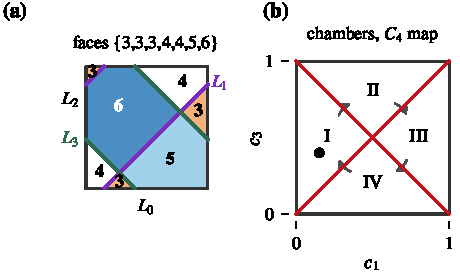
\includegraphics[width=\columnwidth]{figs/fig3.pdf}
\caption{(a)~Coarse arrangement of one straight line per family on the torus (unit square, opposite sides identified). The numbers give the number of sides of each face, which is the coordination of the corresponding defect vertex. (b)~Offset space $(c_1,c_3)$. Triple-point walls divide it into four chambers that the $C_4$ map $(c_1,c_3)\mapsto(c_3,1-c_1)$ permutes. The dot marks the offsets used in (a).}
\label{fig:arr}
\end{figure}

\subsection{Energetics and the instability of the quasicrystal}

Figure~\ref{fig:facet} compares an approximant, with the lines of the de~Bruijn multigrid spread evenly, and a faceted tiling of identical composition (squares:rhombi $=17:24$). In the approximant $66\%$ of sites have $z\ne4$, at a cost of $+0.012J$ per site relative to $e_{\rm sq}$. In the faceted tiling only the quintet remains. Its period energy obeys
\begin{equation}
E_p(N)=n_q\,\eps_5-\frac{c_{\rm C}}{\sqrt N},
\label{eq:Ep}
\end{equation}
where $n_q$ is the number of quintets per period [Fig.~\ref{fig:facet}(c)]. LSWT gives $\eps_5\simeq0.035J$, and $c_{\rm C}\simeq2$ coincides with the Casimir coefficient of the square-lattice torus (compare Ref.~\cite{Jagannathan2013}). The apparent growth of the period energy with system size is therefore a finite-size effect of the Goldstone modes, not a defect interaction. QMC gives $\eps_5=0.03\pm0.01\,J$ after separating the Casimir term with two system sizes.

In an open quasiperiodic patch of $741$ sites, $99$ of the $185$ interior single flips lower the LSWT energy, and the most favorable ones remove the $z=8$ hubs, the non-interval structure of Theorem~1. The quasiperiodic state is therefore not even a local minimum in LSWT, consistent with the energy lowering by phason disorder found in QMC~\cite{Szallas2009}. The zero-field ground state at fixed composition is faceted, with $O(1)$ defects per period.

\begin{figure*}[t]
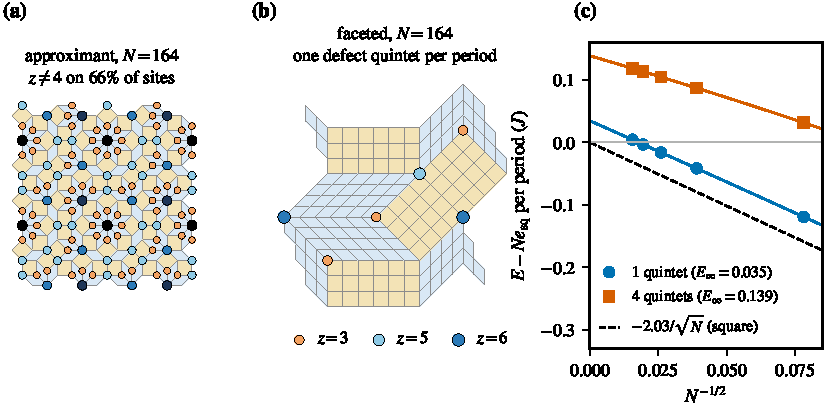
\includegraphics[width=\textwidth]{figs/fig2.pdf}
\caption{(a)~Approximant obtained from evenly spread multigrid lines, line numbers $(6,4,6,4)$. (b)~Faceted tiling of the same composition. The lines of each family are gathered into one band, leaving single-type domains and one defect quintet per period. Colored vertices have $z\neq4$. (c)~Period energy relative to the square lattice. Lines are fits to Eq.~\eqref{eq:Ep} with an additional $1/N$ term. The two-band construction contains four quintets and its asymptote is $4.0$ times that of the one-band construction. The slope matches the Casimir term of the square-lattice torus (dashed).}
\label{fig:facet}
\end{figure*}

%=====================================================================
\section{Magnetic field: budget lines and the staircase}\label{sec:field}
%=====================================================================

\subsection{The thermodynamic limit as a linear program}

Because folds are free and squares can be placed in any $z=4$ domain, a large system can separate into homogeneous phases at no extensive cost. We characterize a phase $P$ per rhombus by its polarization $\tau_P$, its number of squares $\sigma_P$, and its zero-point cost $\eps_P$ relative to the square lattice. Unpolarized regions cant in the field and gain $\Delta e_{\rm sq}(h)\simeq-\chi h^2/2$ per site. Collinear ferrimagnetic phases do not cant until their spin-flop gap $\Delta_+$ is reached, which for all relevant phases exceeds $0.18J$. The energy per rhombus is then
\begin{equation}
\min_{x_P\ge0}\sum_P x_P\Big[\eps_P+|\Delta e_{\rm sq}|(1+\sigma_P)-\frac h4\tau_P\Big],
\label{eq:LP}
\end{equation}
subject to $\sum_Px_P\le1$ and $\sum_Px_P\sigma_P\le S_\square/R$. The optimum jumps between vertices of a polytope, so $m(h)$ is a staircase. A smooth ramp would require a continuous family of phases with strictly convex $\eps(\tau)$. Parallel ribbons repel too weakly ($\simeq0.0016J/d^2$ per rhombus) for such a family to be selected.

\subsection{Plateau values as saturated budgets}

In the $(c,m)$ plane, a mixture of phases lying on a common straight line stays on that line. A family of cheap phases on a line therefore produces a plateau at the corresponding magnetization for any global composition. Exact counting provides the lines (Fig.~\ref{fig:budget}). Equation~\eqref{eq:mmax}, $m=(1-c)/2$, is saturated when every rhombus has $\tau=+1$. A minority vertex with $z=5$ whose star consists of two acute corners and three square corners consumes three square corners per unit charge, which gives $m\le c/3$. Equation~\eqref{eq:kappa} gives $m\le1/5$ for $\kappa_B\le1$. The $z=5$ crystal ($c=3/5$, $m=1/5$) lies at the common intersection of these three lines. Among them only $m=1/5$ is independent of composition, and exceeding it requires net sixfold minority hubs. The same counting gives the hub-free bound of lozenge tilings~\cite{Yoo2026}; there the moment is normalized as $|N_A-N_B|/2N$ and the bound reads $(3/5)$ of the dice value, which is $m=1/5$ in the present convention.

\begin{figure}[t]
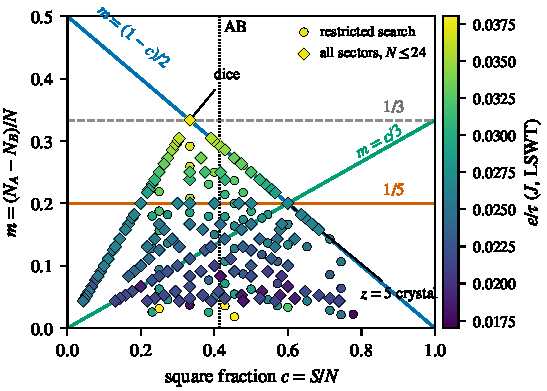
\includegraphics[width=\columnwidth]{figs/fig4.pdf}
\caption{Budget lines in the plane of square fraction $c$ and magnetization $m$, together with the enumerated homogeneous phases, colored by their LSWT cost per unit moment. Circles: orientation-restricted search of earlier work; diamonds: phases within $10^{-3}J$ per rhombus of the lower envelope in the search over all winding sectors with $N\le24$. Mixing phases moves along straight lines, so families of cheap phases on a budget line produce plateaus at the composition of the sample (dotted vertical line: Ammann--Beenker, $c=\sqrt2-1$).}
\label{fig:budget}
\end{figure}

\subsection{Carriers: ribbons, turns, and hubs}

In a region with three families every rhombus lies on a ribbon of the third family. The ribbon is a staircase of horizontal and vertical steps $\sigma_k=\pm1$ across a square background [Fig.~\ref{fig:ribbon}(a)]. Following the sublattice parity along the ribbon gives the exact mapping
\begin{equation}
\tau_k=(-1)^k\sigma_k .
\end{equation}
Straight runs are therefore unpolarized, and only turns carry moment. A turn ($\tau_k=\tau_{k+1}$) is a curvature dipole, a $z=3$/$z=5$ pair with moment $\pm1/2$ whose sign is set by its position. Runs of odd length preserve the sign. The ribbon thus maps onto an Ising chain,
\begin{equation}
H_{\rm rib}=\sum_k\big[\eps_t n_k+J_1n_kn_{k+1}\big]-\frac h4\sum_k\tau_k,
\end{equation}
where $n_k=\tfrac12(1+\tau_k\tau_{k+1})$ counts turns,
and the parameters are the turn energy $\eps_t\simeq0.018J$ and nearest-turn repulsion $J_1\simeq0.009J$ in LSWT [Fig.~\ref{fig:ribbon}(b)]. Turns at larger separation interact by less than $5\times10^{-4}J$. Fully turning ribbons at spacing three form the $z=5$ crystal, and at spacing one the dice lattice [Fig.~\ref{fig:phases}(c),(d)].

\begin{figure*}[t]
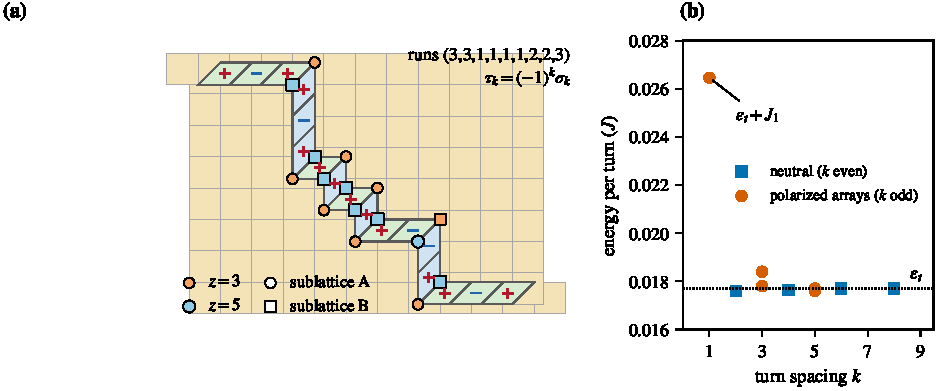
\includegraphics[width=\textwidth]{figs/fig5.pdf}
\caption{(a)~A ribbon of the third family in a square background. Signs give the rhombus polarization $\tau_k=(-1)^k\sigma_k$. Each turn creates a $z=3$/$z=5$ dipole; marker shapes give the sublattice. Odd runs keep the moment sign, and the even run reverses it. (b)~Energy per turn for words $H^kV^k$. Neutral ribbons ($k$ even) and dilute polarized arrays ($k\geq3$) both give $\eps_t\simeq0.0177J$. Adjacent turns ($k=1$) cost an additional $J_1$.}
\label{fig:ribbon}
\end{figure*}

Ribbons are not the only carriers. An exhaustive search over all winding sectors of periodic tilings with up to $24$ tiles per cell (Appendix~\ref{app:search}) reveals rhombus-rich, partially polarized phases (Figs.~\ref{fig:budget} and~\ref{fig:phases}). The cheapest carrier per unit moment is an isolated sixfold hub flanked by two threefold sites in a background with $\sigma=1/2$ [Fig.~\ref{fig:phases}(a)]. The next carriers are dilute $z=3$/$z=5$ pairs in three-family regions [Fig.~\ref{fig:phases}(b)], and at higher fields hub-free crystals with $z=3$ on every majority defect and $z=5$ on every minority defect, which lie on the line $m=1/5$ [Fig.~\ref{fig:phases}(c)]. This is unexpected from the curvature picture, which would favor charge-one carriers, and shows that the cost of a carrier depends on its background as much as on its charge.

The site colors in Fig.~\ref{fig:phases} show how the field sorts the curvature charges. Every majority site, with $z\le4$, carries a moment along $h$, and every minority site, with $z\ge4$, carries a moment against it, as in the lozenge case. The magnitude, however, is set less by $z$ than by the polarization of the phase [Fig.~\ref{fig:phases}(e)]. A threefold rim carries $\langle S_i^z\rangle=0.31$ next to an isolated hub, close to the square-lattice value $0.303$, but $0.43$ in the dice lattice; minority hubs go from $-0.33$ to $-0.36$. The ferrimagnetic moment gaps the moment-raising magnons and suppresses the zero-point reduction on every site of the phase. Near an isolated hub the threefold rims are even slightly less ordered than the fourfold sites ($0.311$ versus $0.322$), because the bonds around a rim fluctuate more strongly. Both observations are the site-level counterpart of the bond-fluctuation compensation discussed in Sec.~\ref{sec:hartree}.

\begin{figure*}[t]
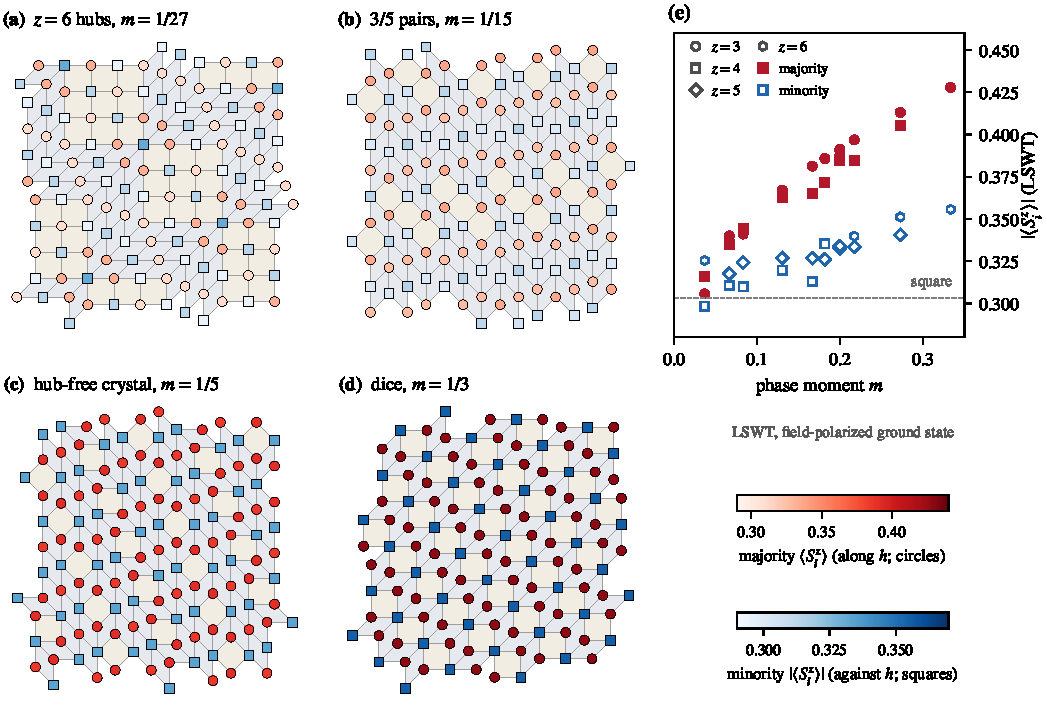
\includegraphics[width=\textwidth]{figs/fig6.pdf}
\caption{Homogeneous phases that enter the staircase, colored by the local moment $\langle S_i^z\rangle$ in the field-polarized ground state (LSWT, converged supercells). Majority sites (circles, red scale) carry moments along $h$, and minority sites (squares, blue scale) against it; the two color scales are separate and start at $0.29$, below the square-lattice value $0.303$, so that differences between sites are visible. All symbols have the same size; the coordination of a site can be read from the tiles around it. The moments do not change within a plateau. (a)~Isolated sixfold hubs in a rhombus-rich background, the first carriers in a field. (b)~A three-family crystal of dilute $z=3$/$z=5$ pairs ($\sigma=1/4$), the first window phase. (c)~A hub-free crystal ($\sigma=1/4$) with $z=3$ on every majority defect and $z=5$ on every minority defect, on the line $m=1/5$. (d)~The dice lattice. (e)~Mean $|\langle S_i^z\rangle|$ for each sublattice and coordination versus the moment $m$ of the phase, for the phases on the $N_{\max}=24$ ground-state path. Filled (open) symbols: majority (minority) sites. Dashed line: square lattice.}
\label{fig:phases}
\end{figure*}

\subsection{The magnetization staircase}

Figure~\ref{fig:mh} shows $m(h)$ for the Ammann--Beenker composition with phase energies taken from QMC. The candidate set is defined by a search depth: it contains every periodic tiling whose primitive cell has at most $N_{\max}$ tiles, in every winding sector (Appendix~\ref{app:search}). Every phase that appears on the ground-state path for any depth was simulated directly with three independent seeds ($40$ phases in total; Appendix~\ref{app:qmc}). Phases that never reach the path enter with the ratio of Eq.~\eqref{eq:fit}. To decide which steps are resolved, we redrew every phase energy $4000$ times within its error (statistical error of the seeds for simulated phases, the $0.018$ rms of Eq.~\eqref{eq:fit} otherwise) and recorded for each plateau the fraction of redraws in which it is present and the spread of its onset field [Fig.~\ref{fig:mh}(b)].

Three features are present in at least $97\%$ of the redraws at every depth (Table~\ref{tab:robust}). Magnetization sets in at $h_c\simeq0.071J$ through isolated sixfold hubs ($m\simeq0.033$). A plateau at exactly $m=1/5$ begins at $h\simeq0.18$--$0.19J$ and lasts to $h\simeq0.25J$; it is carried by the hub-free crystal with $\sigma=2/3$ together with a little of the $z=5$ crystal. The curve ends with a jump at $h\simeq0.266J$ into dice domains coexisting with a crystal of $z=5$ and $z=6$ minority sites, where $m$ reaches $m_{\max}=1-1/\sqrt2$. Compared with the restricted search used earlier, the plateau at $m\simeq0.190$ is replaced by the exact bound $m=1/5$, and the final jump moves from $0.245J$ to $0.266J$. The onset carries an additional systematic uncertainty of about $0.005J$ from finite-size effects (Appendix~\ref{app:qmc}). Between $h\simeq0.09J$ and $0.18J$ (the window) the staircase changes with the search depth. We discuss this window separately below.

\begin{table*}[t]
\caption{Features of the QMC-based staircase that are independent of the search depth. Brackets give the 16--84\% range of the onset field over $4000$ redraws of the phase energies; $P$ is the fraction of redraws in which the plateau is present. ``Restricted'' is the orientation-restricted search of earlier work.}
\label{tab:robust}
\begin{ruledtabular}
\begin{tabular}{lccc}
search & onset $h_c/J$ & plateau $m=1/5$: onset, $P$ & final jump $h/J$\\
\hline
restricted & $0.071\,[0.065,0.075]$ & absent ($m=0.190$ instead) & $0.245\,[0.243,0.247]$\\
$N_{\max}=16$ & $0.071\,[0.066,0.075]$ & $0.180\,[0.178,0.182]$, $1.00$ & $0.266\,[0.263,0.271]$\\
$N_{\max}=21$ & $0.071\,[0.065,0.075]$ & $0.182\,[0.179,0.188]$, $1.00$ & $0.266\,[0.263,0.272]$\\
$N_{\max}=24$ & $0.071\,[0.065,0.075]$ & $0.192\,[0.188,0.197]$, $0.97$ & $0.267\,[0.263,0.274]$\\
\end{tabular}
\end{ruledtabular}
\end{table*}

\begin{figure*}[t]
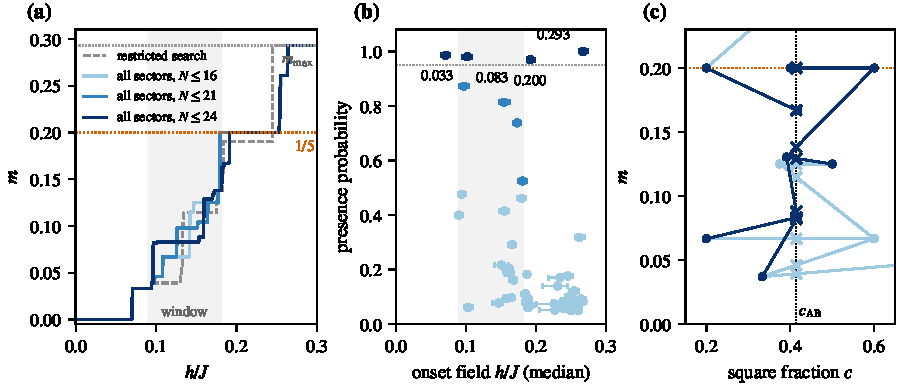
\includegraphics[width=\textwidth]{figs/fig7.pdf}
\caption{Magnetization curve for the Ammann--Beenker composition with QMC phase energies, including the canting of unpolarized regions. (a)~Central staircase for the orientation-restricted search of earlier work (dashed) and for all winding sectors with at most $N_{\max}=16$, $21$, $24$ tiles per cell. Dotted lines mark $m=1/5$ and $m_{\max}$; the shaded band is the window in which the staircase depends on $N_{\max}$. (b)~Presence probability of each plateau over $4000$ redraws of the phase energies ($N_{\max}=24$) versus its median onset field; bars give the 16--84\% range of the onset. Labels give $m$ for plateaus present in at least $95\%$ of redraws. (c)~Tie lines of the phase pairs selected on plateaus wider than $0.004J$, in the $(c,m)$ plane, for $N_{\max}=16$ (light) and $24$ (dark). Each plateau value is the crossing of a tie line with the sample composition $c_{\rm AB}$ (crosses), Eq.~\eqref{eq:tie}. Only tie lines along $m=1/5$ give a value independent of the selected pair.}
\label{fig:mh}
\end{figure*}

\subsection{The intermediate window: finite-cell results}

Inside the window the selected phases and plateau values depend on $N_{\max}$ [Fig.~\ref{fig:mh}(a)]. For $N_{\max}=16$ the main plateau is $m\simeq0.067$ ($h\simeq0.11$--$0.14J$, presence $0.89$), a mixture of two three-family crystals with $\sigma=1/4$ and $3/2$ that share the same graph of dilute $z=3$/$z=5$ pairs [Fig.~\ref{fig:phases}(b)]. For $N_{\max}=21$ a crystal with $\sigma=2/3$ takes over above $0.126J$ and gives $m\simeq0.098$. For $N_{\max}=24$ a single crystal with $\sigma=5/7$ fills $99\%$ of the rhombi from $0.10J$ to $0.15J$ and gives a plateau at $m\simeq0.083$ that is present in $98\%$ of the redraws. The other window plateaus have presence probabilities between $0.5$ and $0.9$ at every depth and are not resolved. Each deepening lowers the energy in the window by up to $6\times10^{-4}J$, $4\times10^{-4}J$, and $6\times10^{-4}J$ per rhombus in the three successive steps of Fig.~\ref{fig:mh}(a). Outside the window the changes are smaller, at most $3\times10^{-4}J$ from $N_{\max}=21$ to $24$, and they do not move the features of Table~\ref{tab:robust}.

\subsection{Why the window need not converge}

Three properties of the linear program~\eqref{eq:LP}, two of them exact, explain this behavior and suggest that it persists at every finite depth.

\paragraph*{Both resources bind.} Inside the window the whole sample is polarized, so both constraints of Eq.~\eqref{eq:LP} are saturated, $\sum_Px_P=1$ and $\sum_Px_P\sigma_P=s_0$ with $s_0=S_\square/R=1/\sqrt2$ for the Ammann--Beenker composition. The energy per rhombus is then $E(h)=\min_\tau[\bar\eps(s_0,\tau)-h\tau/4]$, where $\bar\eps(\sigma,\tau)$ is the lower convex envelope of the points $(\sigma_P,\tau_P,\eps_P)$. The magnetization is the slope of the Legendre transform, so each vertex of the one-dimensional section $\bar\eps(s_0,\cdot)$ is a plateau.

\paragraph*{No crystal has the sample composition.} Every periodic phase has a rational ratio $\sigma_P=S/R$, whereas $s_0$ is irrational. The section at $s_0$ is therefore never a crystal; it is a tie line between two phases (or one phase and unpolarized facets) on either side of $s_0$. In the per-site plane of Fig.~\ref{fig:budget} a tie line between phases at $(c_1,m_1)$ and $(c_2,m_2)$ crosses the sample composition $c_{\rm AB}=\sqrt2-1$ at
\begin{equation}
m=m_1+(m_2-m_1)\frac{c_{\rm AB}-c_1}{c_2-c_1},
\label{eq:tie}
\end{equation}
so the plateau value depends on which pair is selected. The exception is a tie line along a horizontal budget line, $m_1=m_2$: then $m$ does not depend on the pair at all [Fig.~\ref{fig:mh}(c)]. This is why the plateau $m=1/5$ is robust. Every phase that carries it (the $z=5$ crystal and the hub-free crystals with $\sigma=1/4$, $1/2$, $2/3$, and $1$, all with $z=3$ on the majority and $z=5$ on the minority sublattice) lies on the line $m=1/5$, and so does every mixture of them. The same holds for $m_{\max}$, which lies on $m=(1-c)/2$.

\paragraph*{Approximants keep appearing.} If the cost of the cheapest crystals at fixed $\tau$ is a strictly convex function of $\sigma$ with curvature $\kappa_\sigma$, a tie line between $\sigma_1<s_0<\sigma_2$ costs $\tfrac12\kappa_\sigma(\sigma_2-s_0)(s_0-\sigma_1)$ more than a crystal at $s_0$. A deeper search finds crystals closer to $s_0$, which replace the tie line and change the plateau. The closest ratios available with at most $R$ rhombi are the convergents of the continued fraction $1/\sqrt2=[0;1,2,2,2,\dots]$, namely $2/3$, $5/7$, $12/17$, $29/41,\dots$, with $|\sigma-s_0|\propto1/R^2$. A further exact constraint fixes where each convergent can first appear. A polarized crystal needs a cell whose periods preserve the sublattices, since a period that exchanges them forces $M=0$. In such a cell Eq.~\eqref{eq:tau} gives $\sum_t\tau_t=2M$, so the number of rhombi $R$ is even. A polarized crystal with $\sigma=p/q$ in lowest terms therefore needs $R=q$ for even $q$ and $R\ge2q$ for odd $q$, that is, at least $N=10$, $24$, $58$, and $140$ tiles for the four convergents above. The window phases follow this sequence. Crystals with $\sigma=2/3$ ($N=10$ and $20$) dominate for $N_{\max}=21$. The first crystal with $\sigma=5/7$ appears at exactly $N=24$ and takes over at $N_{\max}=24$. As a direct check, all $7\times10^4$ tilings in the $55$ sectors with $\sigma=12/17$ and $N=29$, whose periods necessarily exchange the sublattices, have $M=0$. The next polarized convergent requires $N\ge58$, far beyond an exhaustive search, and successive thresholds grow by the factor $1+\sqrt2$. Every finite search therefore stops at some convergent. Because $s_0$ is irrational, the sequence never ends, and each new convergent can add or move vertices of $\bar\eps(s_0,\cdot)$. The plateau values in the window are therefore not expected to converge as $N_{\max}$ grows.

What does converge is the energy. $E(h)$ decreases monotonically with $N_{\max}$ and is bounded below, and the energy changes are already of order $10^{-4}J$ per rhombus. Hence $m(h)$ converges at every field where the limiting $E(h)$ is differentiable. The limit is set by structures whose composition equals $s_0$ exactly, either quasiperiodic arrangements of the same local carriers or coexisting approximants separated by interfaces. No finite cell represents these structures, and whether the limit is a devil's staircase or a continuous ramp cannot be decided from cells of the present size. Two statements are nevertheless model independent. First, any plateau that survives in the window must lie on a composition-independent budget line or come from a sequence of approximants whose plateau values converge. Second, for a periodic approximant of the tiling with a rational composition, the window becomes a finite staircase set by that approximant, while the onset, the plateau $m=1/5$ and the final jump do not move.

\subsection{Energy balance along the ground-state path}

Within a collinear phase the exchange energy and the moment do not depend on the field at all, because $[H_J,S^z_{\rm tot}]=0$ and the spin-flop gap $\Delta_+$ exceeds the fields of interest. The Zeeman energy of the phase is exactly linear, $-hSM_P$. Only the unpolarized $z\equiv4$ facets respond continuously, with an exchange cost $\chi h^2/2$ and a Zeeman gain $-\chi h^2$ per site. Along the ground-state path the exchange energy is therefore a staircase whose risers obey
\begin{equation}
\Delta E_{\rm ex}(h_i)=h_i\,\Delta\langle S^z_{\rm tot}\rangle ,
\label{eq:balance}
\end{equation}
so that at every step field the additional zero-point cost of the new structures is paid exactly by the Zeeman gain. Figure~\ref{fig:path} shows this balance for the Ammann--Beenker composition, with QMC phase energies for $N_{\max}=24$ and the split into normal ($zz$, along $h$) and in-plane ($xx+yy$) parts measured by SSE in the Lieb sector of each phase.

Three features stand out. First, the onset at $h\simeq0.071J$ converts about $88\%$ of the sites into hub domains at once, yet the moment rises only to $m\simeq0.03$ [Fig.~\ref{fig:path}(a)]. The step in the exchange components is nevertheless large: the normal energy drops from $-0.22$ to $-0.29J$ per site and the in-plane energy rises from $-0.45$ to $-0.38J$ [Fig.~\ref{fig:path}(b)]. In the canted facets the staggered axis lies perpendicular to $h$, whereas in a collinear Lieb domain it lies along $h$. The first step is thus primarily a reorientation of the staggered axis, and the moment is a small by-product. Second, from $h\simeq0.10J$ on, the whole sample consists of polarized phases. The normal and in-plane energies approach each other step by step and cross at $h\simeq0.18J$ (16--84\% range $0.174$--$0.188J$), where the hub-free crystals of the $m=1/5$ plateau take over. Which approximant crystals fill the window is uncertain [hatched in Fig.~\ref{fig:path}(a)], but the exchange and Zeeman energies are not: alternatives that compete in the window differ by less than $5\times10^{-4}J$ per site in total energy. Third, after the final jump the sample is $33\%$ dice and $67\%$ of a crystal with $z=5$ and $z=6$ minority sites, by site. Its normal and in-plane energies, $-0.36$ and $-0.28J$, are close to those of the dice phase in the lozenge study. The exchange energy rises by $0.026J$ per site in total, the Zeeman energy falls in larger steps, and their sum is a smooth concave function of $h$, as required by $\partial^2E/\partial h^2=-\partial\langle S^z\rangle/\partial h\le0$ [Fig.~\ref{fig:path}(c)].

\begin{figure*}[t]
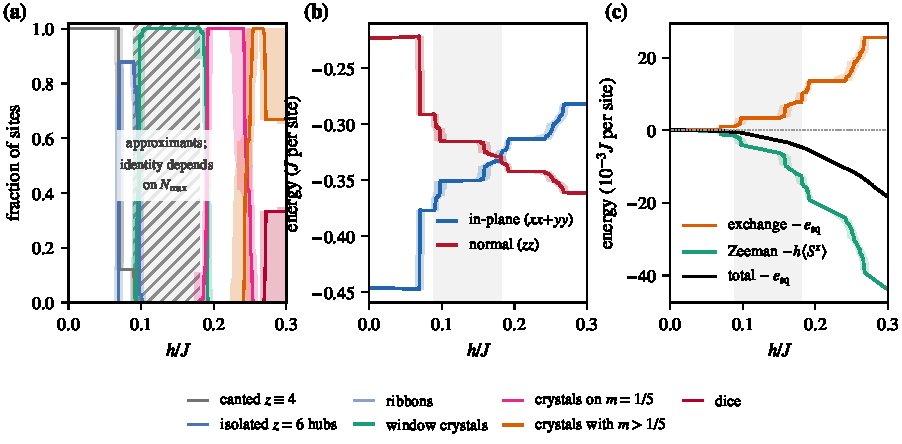
\includegraphics[width=\textwidth]{figs/fig_path.pdf}
\caption{Energy balance along the QMC ground-state path for $N_{\max}=24$ (Ammann--Beenker composition) and its uncertainty. Lines are medians and shaded bands the 16--84\% range over $500$ redraws of the phase energies, with the same error model as Fig.~\ref{fig:mh}(b). (a)~Fraction of sites in each class of homogeneous phases; gray: unpolarized $z\equiv4$ facets that cant in the field. ``Window crystals'' are the approximant crystals of Sec.~\ref{sec:field}; within the hatched window their identity changes with $N_{\max}$ and is not resolved, although their total fraction is. ``Crystals on $m=1/5$'' are the hub-free crystals and the $z=5$ crystal. Wide bands near $0.19J$ and $0.24$--$0.27J$ show where the step fields are uncertain. (b)~Normal ($zz$, along $h$) and in-plane ($xx+yy$) exchange energy per site. The split of each simulated phase is measured by SSE in its Lieb sector ($\beta J=300$); for phases that appear only in some redraws it is interpolated linearly in the phase moment (rms deviation $0.003$ of the $zz$ share). The canted facets start from $e_{\rm sq}/3$ and $2e_{\rm sq}/3$ and use the split of $L=16$ fixed-$S^z$ sectors. (c)~Exchange energy relative to $e_{\rm sq}$, Zeeman energy, and their sum. The band of the total energy is narrower than the line: the redraws change which structures are selected, but hardly the energy balance.}
\label{fig:path}
\end{figure*}

%=====================================================================
\section{Quantum corrections depend on charge density}\label{sec:hartree}
%=====================================================================

We computed phase energies with a stochastic series expansion that builds and flips all loops deterministically, without a length cap~\cite{Sandvik2010}. It is validated against exact diagonalization (Appendix~\ref{app:qmc}). The ratio $r=\eps_{\rm QMC}/\eps_{\rm LSWT}$ is not universal. It ranges from $0.86$--$0.89$ for isolated hubs (depending on cell size) to $1.25$--$1.30$ for the $z=5$, hub-free, and dice crystals, and it rises monotonically with the mean minority charge $\kappa_B$ [Fig.~\ref{fig:ratio}(a)].

\subsection{Bond-fluctuation formulation}

In terms of the quadratures of the Holstein--Primakoff bosons~\cite{Holstein1940} in the rotated frame, the zero-point fluctuation of bond $b=(ij)$ is
\begin{equation}
\delta_b=\tfrac12-\tfrac14\big\langle(q_i+q_j)^2\big\rangle-\tfrac14\big\langle(p_i-p_j)^2\big\rangle .
\end{equation}
The LSWT energy is $E_1=-J\sum_b(S^2+2S\delta_b)$. The first magnon-interaction correction, of order $S^0$ (the Hartree or Oguchi term~\cite{Oguchi1960}), is $E_2=-J\sum_b\delta_b^2$, so that $E\simeq-J\sum_b(S+\delta_b)^2$. For the square lattice this gives $\delta=0.0790$ and $E_2/N=-0.0125J$, in agreement with the spin-wave series~\cite{Hamer1992}. With $w_b=\delta_b-\delta_{\rm sq}$,
\begin{equation}
r_H-1=\frac{\Delta E_2}{\Delta E_1}\simeq\frac{\langle\delta+\delta_{\rm sq}\rangle_--f\,\langle\delta+\delta_{\rm sq}\rangle_+}{2S(1-f)},
\label{eq:rH}
\end{equation}
with the compensation ratio $f=\sum_{w_b>0}w_b\big/\sum_{w_b<0}|w_b|$,
where $\langle\cdot\rangle_-$ averages over bonds with suppressed fluctuations (around hubs and in polarized regions) and $\langle\cdot\rangle_+$ over bonds with enhanced fluctuations (around threefold rims).

\subsection{Interpretation}

The harmonic cost of a phase is a net suppression of bond fluctuations. The Hartree term weights every bond by $\delta_b+\delta_{\rm sq}$ and therefore counts the enhanced bonds more heavily. In phases with dilute charges, suppression and enhancement nearly compensate ($f\simeq0.85$ for isolated hubs). The small harmonic cost is then reduced further and $r<1$. As the charge density grows, the ferrimagnetic moment gaps the moment-raising magnon branch and suppresses fluctuations everywhere [compare the local moments in Fig.~\ref{fig:phases}(e)]. Then $f\to0$ and $r-1\to(\bar\delta+\delta_{\rm sq})/2S\simeq0.15$. This is why the ratio follows $\kappa_B$. Across the eight phases of the fit set,
\begin{equation}
r_{\rm QMC}=1.114+1.152\,(r_H-1),
\label{eq:fit}
\end{equation}
with correlation $0.989$ and rms deviation $0.018$ [Fig.~\ref{fig:ratio}(b)]. The constant offset collects higher-order terms that are nearly uniform across phases.

\subsection{Blind test}

For four phases outside the fit set we computed $r_H$ from LSWT correlators and recorded the prediction of Eq.~\eqref{eq:fit} before running QMC. The predicted values $1.159$, $1.220$, $1.216$, $1.131$ compare with the measured $1.165$, $1.222$, $1.222$, $1.113$ (stars in Fig.~\ref{fig:ratio}), all within $0.018$. The search over all winding sectors provided a second, larger test. For each of the $31$ new phases that reached a ground-state path we recorded the prediction before simulating it (triangles in Fig.~\ref{fig:ratio}). The rms deviation is $0.039$. The mean deviation is $+0.020$: Eq.~\eqref{eq:fit} slightly underestimates the ratio of hub-free crystals with $\kappa_B\simeq1$. The largest deviations ($0.17$ and $0.07$) belong to the two phases with the largest finite-size corrections. The Hartree picture thus captures the trend across phases, which is what decides the staircase, but not the last few percent. For this reason every phase on a ground-state path in Fig.~\ref{fig:mh} was simulated directly, and Eq.~\eqref{eq:fit} is used only to screen the remaining candidates.

\begin{figure*}[t]
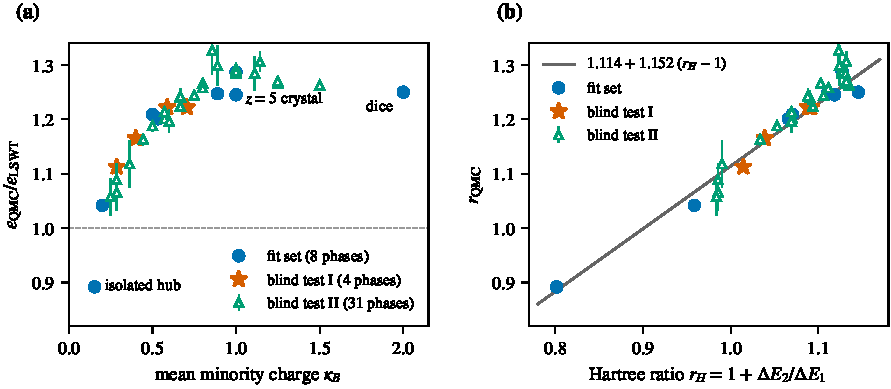
\includegraphics[width=\textwidth]{figs/fig8.pdf}
\caption{(a)~Ratio of QMC to LSWT phase energies versus the mean minority charge $\kappa_B$. (b)~The same ratio versus the Hartree estimate $r_H$ of Eq.~\eqref{eq:rH}, with the fit of Eq.~\eqref{eq:fit}. Stars (blind test I) and triangles (blind test II, phases from the search over all winding sectors) are phases outside the fit set whose ratios were predicted before the simulation; error bars include finite-size uncertainty.}
\label{fig:ratio}
\end{figure*}

%=====================================================================
\section{Discussion}\label{sec:disc}
%=====================================================================

\paragraph*{What is model independent.} Bipartiteness, classical degeneracy, the identities~\eqref{eq:tau} and~\eqref{eq:kappa}, the interval classification, the exactness of domain energies, cost-free folds, the topological quintet, the budget lines, and the energy balance~\eqref{eq:balance} at every step all follow from counting and symmetry. They hold for any spin length and any interaction that depends only on the exchange graph. The approximation enters only through phase energies, which decide which budget line is realized and at what field. The plateau $m=1/5$ and the final jump appear in LSWT as well as in QMC; the energetics moves their fields, and it decides which approximants fill the window.

\paragraph*{Where the model meets experiment.} Magnetization plateaus are usually traced to frustration~\cite{Kageyama1999,Honecker2004} or to a coupling of the spins to lattice distortions~\cite{Penc2004,Vekua2006}. Here the lattice itself is the degree of freedom, and the plateaus count curvature charges. The predictions concern dependencies. The upper plateau bounds move with composition as $c/3$ and $(1-c)/2$, so approximants with different square fractions should shift them along these lines, while the plateau at $m=1/5$ should not move. Below it, a periodic approximant with rational composition should show a finite staircase whose plateau values follow Eq.~\eqref{eq:tie} for the crystals that fit its composition, so that two approximants of the same tiling family can differ there while agreeing on the onset, on $m=1/5$, and on the final jump. The onset field is set by the cost of an isolated hub divided by its moment, $\simeq0.07J$. Exchange anisotropy gaps the magnons and cuts off the long-range parts of carrier interactions beyond $\xi=c_{\rm sw}/\Delta$, which sharpens the steps rather than smearing them. Natural platforms are systems in which the tiling is itself dynamical, such as artificial spin lattices~\cite{Skjaervo2020}, reconfigurable tweezer arrays~\cite{Browaeys2020,Scholl2021}, and atom-by-atom assembled structures~\cite{Khajetoorians2019}.

\paragraph*{Interactions between carriers.} Uncompensated moments on opposite sublattices attract through a magnon Casimir-type force, the vacuum polarization of the Lieb charge, which scales as $\lambda_1\lambda_2/d^2$ per unit length for lines. Moments on the same sublattice repel weakly. A distance-independent global term $\propto|\mu|/N$, with $\mu=(N_A-N_B)/2$, must be removed before pair forces can be measured. These results will be reported separately. Here they enter only through the weak repulsion of parallel ribbons, which keeps the steps sharp.

\paragraph*{Open problems.} Minimality of the quintet for curved band arrangements should follow from minimal-position theory for curves on the torus~\cite{HassScott1985} together with a finite enumeration. The window between the onset and $m=1/5$ calls for a treatment of incommensurate composition: the cost of the cheapest crystals as a function of $\sigma$ near $1/\sqrt2$, interfaces between approximants, and quasiperiodic arrangements of $z=3$/$z=5$ carriers would decide whether its limit is a devil's staircase~\cite{BakBruinsma1982} or a ramp. At finite temperature, facets carry only subextensive entropy, so the faceted state should melt by dissociation of quintets rather than by roughening of facets~\cite{Henley1991}. Pokrovsky--Talapov-type behavior~\cite{Pokrovsky1979} may appear wherever a continuous family of phases becomes relevant. The fivefold case has ten interval classes and a non-bipartite $C_5$ subtlety that deserves separate study.

\paragraph*{Summary.} Quantum fluctuations select the exchange graph of eightfold rhombus tilings in a way that is largely fixed by geometry. At zero field they produce exact square-lattice facets with a topologically protected defect quintet. In a field they produce a staircase whose plateau bounds are linear budgets of curvature charge. The plateaus that survive every search lie on composition-independent budget lines; the others are set by rational approximants of an irrational composition and change with cell size. At every step the zero-point cost of the new structures is balanced exactly by the Zeeman gain, and the first step mainly turns the staggered axis along the field. The quantum corrections to its energetics are governed by how strongly bond fluctuations compensate.

\begin{acknowledgments}
This research was supported by the National Research Foundation (NRF) of Korea funded by the Korean Government (NRF-2023R1A2C1006050). Claude (Anthropic; Claude Opus 5.5, November 2026) was used to derive and check analytic results, to write the analysis and plotting code, to run numerical tests and to draft and edit the text.
\end{acknowledgments}

\section*{Data availability}
The QMC and spin-wave codes, the winding-sector enumeration, the phase energies, all QMC runs with their seeds, the Hartree predictions recorded before each simulation, and the scripts that produce the figures are openly available at \url{https://github.com/cywon-commits/eightfold-tiling-qmc}. The full lists of enumerated tilings (several hundred megabytes) can be regenerated with the included scripts and are available from the author on request.

\appendix

\section{Proofs}\label{app:proofs}
\paragraph*{Theorem 1.} The eight directions $\pm\mathbf v_j$ in angular order carry family labels $1,2,3,4,1,2,3,4$. A bipartition $P|Q$ with interval parts colors them in exactly four blocks $PP\,QQ\,PP\,QQ$ (or $P\,QQQ\,P\,QQQ$ for stars). Consecutive edges must change color and are at most $135^\circ$ apart, so each block is visited once and $z=4$. A non-interval split gives eight singleton blocks, and gaps of $45^\circ$ or $135^\circ$ that sum to $360^\circ$ give $z=4$, $6$, or $8$.
\paragraph*{Extended domains.} Three ribbons that cross pairwise enclose a triangle that contains a threefold cell, by induction on the number of enclosed cells. Ribbon $j$ has mean direction in the arc $[\frac{\pi}{4}j,\frac{\pi}{4}(j+2)]$. A defect-free uniform domain contains at most two mean directions, and the arcs of a group must overlap. The overlaps are intervals of positive length for $\{12|34\}$ and $\{14|23\}$ and single points for $\{13|24\}$, which forces a family to vanish.
\paragraph*{Theorem 2.} $P$-ribbons do not cross each other, nor do $Q$-ribbons. Inside a domain each $P$-ribbon crosses each $Q$-ribbon exactly once, which defines the grid indices $(m,n)$.
\paragraph*{Theorem 3.} With $c_0=c_2=0$, the walls listed in the text bound four triangular chambers. In the chamber $0<c_1<c_3$, $c_1+c_3<1$ the seven faces can be listed explicitly [Fig.~\ref{fig:arr}(a)], and the rotation $(x,y)\mapsto(-y,x)$ maps chamber to chamber while preserving face sizes.

\section{Spin waves, canting, and spin-flop gaps}\label{app:sw}
In the rotated frame $H_2=\sum_iA_ia_i^\dagger a_i+\sum_{\langle ij\rangle}B_{ij}(a_ia_j+{\rm h.c.})$ with $A_i=JSz_i$ and $B_{ij}=JS$. The frequencies are $\omega_n=[{\rm eig}(K^{1/2}MK^{1/2})]^{1/2}$~\cite{Colpa1978} with $K=A+B$ and $M=A-B$, and $E_1=-JS^2N_b+\frac12(\sum_n\omega_n-{\rm Tr}A)$. Unpolarized facets in a field are treated as the canted square lattice, $\omega_{\mathbf k}=4JS[(1+\gamma_{\mathbf k})(1-\gamma_{\mathbf k}\cos2\theta)]^{1/2}$ with $\sin\theta=h/8JS$~\cite{Zhitomirsky1999}. This gives $\chi_{\rm LSWT}\simeq0.058/J$; we use $\chi\simeq0.065/J$ when calibrating to QMC. The spin-flop gaps of the polarized phases are $0.82J$ (the $z=5$ crystal), $1.50J$ (dice), and at least $0.18J$ (dilute ribbons).

\section{Quantum Monte Carlo}\label{app:qmc}
We use the stochastic series expansion with diagonal updates and a deterministic loop update in which every loop is constructed once per sweep and flipped with probability $1/2$ (with heat-bath probabilities in a field). Loops always close, so no length cap is needed, and a sweep costs time linear in the number of operators. Equilibration uses $\beta$ doubling, and an optional fixed-$S^z$ mode samples one magnetization sector. The code reproduces exact diagonalization for a $12$-site dice cell, a $15$-site $z=5$ cell, and the $4\times4$ square lattice in the sectors $M=0,1,2$ within $1.5$ standard deviations. All phases were simulated at $\beta=300J^{-1}$ in the Lieb sector $S^z_{\rm tot}=S|N_A-N_B|$, with checks at $\beta=600J^{-1}$. Every phase that appears on the ground-state path at any search depth was simulated with three independent seeds on supercells of $360$--$1260$ sites; the error combines the binning errors and the scatter between seeds. The path was recomputed after each round of simulations, and phases that entered it were simulated in turn until every phase on all three paths of Fig.~\ref{fig:mh}(a) had been measured. Finite-size effects are reduced by taking the ratio of QMC and LSWT on the same supercell and multiplying it by the converged LSWT cost, $\eps=\eps_{\rm LSWT}(\infty)\,\eps_{\rm QMC}(L)/\eps_{\rm LSWT}(L)$. Phases first simulated on cells of about $370$ sites were repeated on cells of about $800$ sites. The corrected values change by less than $2\times10^{-4}J$ per rhombus for most phases but by up to $1\times10^{-3}J$ for three crystals of the window whose LSWT cost itself converges slowly. We add the change between the two largest cells (or, for a single cell, the size of the correction) to the error in quadrature. For the hub phase the residual change is $1\times10^{-4}J$. Because the onset field is the hub cost divided by its small moment, $h_c\simeq4\eps_{\rm hub}/\tau_{\rm hub}$ up to the canting term, this moves $h_c$ by about $0.005J$, more than its statistical spread. The redraws of Fig.~\ref{fig:mh}(b) draw every simulated phase energy from a Gaussian with its total error and every other phase energy from a Gaussian of relative width $0.018$ about the value of Eq.~\eqref{eq:fit}, and solve the two-resource program exactly by enumerating its basic solutions. Phase energies use $e_{\rm sq}=-0.669437(5)J$~\cite{Sandvik1997}. The seeds, the reference energy, and the redraws follow the procedure of the lozenge study~\cite{Yoo2026}. The exchange energy splits into $\langle H_{zz}\rangle=JN_b/4-\langle n_{\rm d}\rangle/\beta$ and $\langle H_{xy}\rangle=-\langle n_{\rm o}\rangle/\beta$, where $n_{\rm d}$ and $n_{\rm o}$ count diagonal and off-diagonal operators. Local moments are equal-time averages of $S_i^z$ in the fixed-$S^z$ sector. Against exact diagonalization of the $4\times4$ lattice, the split agrees within $1.5$ standard deviations in the sectors $M=0$ and $2$ (e.g.\ $\langle H_{zz}\rangle=-1.4994J$ exact, $-1.5045(34)J$ SSE, at $M=2$).

\section{Phase search}\label{app:search}
\paragraph*{Winding sectors.} A periodic eightfold tiling is a doubly periodic surface in $\mathbb Z^4$ whose lifted periods $\mathbf T_1,\mathbf T_2$ span a rank-two lattice $\Lambda$. The tiling is valid if and only if all Pl\"ucker minors $p_{jk}=T_{1j}T_{2k}-T_{1k}T_{2j}$ have one sign. Then $p_{jk}$ is the number of tiles of type $(j,k)$ per cell, $N=\sum_{j<k}p_{jk}$, and $S=p_{13}+p_{24}$. We enumerate all non-negative vectors $p$ with $\sum p\le N_{\max}$ that satisfy the Pl\"ucker relation $p_{12}p_{34}-p_{13}p_{24}+p_{14}p_{23}=0$. For each we construct the saturated lattice by integer kernels and then all sublattices of index $\gcd(p)$. Sectors are identified up to ${\rm GL}_2(\mathbb Z)$ (row Hermite normal form) and the eightfold point group (signed permutations of the four coordinates). This gives $741$, $1683$, $3742$, and $5761$ sectors for $N_{\max}=12$, $16$, $21$, and $24$. A brute-force enumeration over all integer period matrices reproduces the list for $N\le3$, and an earlier search restricted to small lifted vectors missed $64$ of the $741$ sectors with $N\le12$.

\paragraph*{Tilings within a sector.} In each sector we build one tiling from a de Bruijn grid on the torus, with lines $T_{1j}s+T_{2j}t\equiv\phi_j$ (mod 1) and generic offsets. Every crossing of families $j,k$ is one tile, and the angle sum at every vertex is checked. Breadth-first search over hexagon flips, with tilings identified up to translation, then enumerates the sector, with a cap of $3000$ tilings. Flip connectivity was checked by building each sector from three random offsets; all landed in the same flip component. All $3742$ sectors with $N\le21$ were exhausted ($8.1\times10^4$ tilings), and $5736$ of the $5761$ sectors with $N\le24$ ($3.2\times10^5$ tilings). Tilings whose graph has $z\equiv4$ are square lattices and have $\eps=0$.

\paragraph*{Screening.} For every composition $(\sigma,\tau)$ the five lowest tilings at a supercell of about $150$ sites were re-evaluated at about $600$ sites. Compositions within $10^{-3}J$ per rhombus of the LSWT lower envelope at some field were evaluated at about $1500$ sites, together with their Hartree ratio. The phases of the earlier, orientation-restricted search are included with their converged energies.

\begin{thebibliography}{99}
\bibitem{Villain1980} J. Villain, R. Bidaux, J.-P. Carton, and R. Conte, Order as an effect of disorder, \href{https://doi.org/10.1051/jphys:0198000410110126300}{J. Phys. (Paris) \textbf{41}, 1263 (1980)}.
\bibitem{Henley1989} C. L. Henley, Ordering due to disorder in a frustrated vector antiferromagnet, \href{https://doi.org/10.1103/PhysRevLett.62.2056}{Phys. Rev. Lett. \textbf{62}, 2056 (1989)}.
\bibitem{Henley2006} C. L. Henley, Order by disorder and gaugelike degeneracy in a quantum pyrochlore antiferromagnet, \href{https://doi.org/10.1103/PhysRevLett.96.047201}{Phys. Rev. Lett. \textbf{96}, 047201 (2006)}.
\bibitem{LiebMattis1962} E. Lieb and D. Mattis, Ordering energy levels of interacting spin systems, \href{https://doi.org/10.1063/1.1724276}{J. Math. Phys. \textbf{3}, 749 (1962)}.
\bibitem{Lieb1989} E. H. Lieb, Two theorems on the Hubbard model, \href{https://doi.org/10.1103/PhysRevLett.62.1201}{Phys. Rev. Lett. \textbf{62}, 1201 (1989)}.
\bibitem{Sandvik1999} A. W. Sandvik, Stochastic series expansion method with operator-loop update, \href{https://doi.org/10.1103/PhysRevB.59.R14157}{Phys. Rev. B \textbf{59}, R14157 (1999)}.
\bibitem{Syljuasen2002} O. F. Sylju\aa sen and A. W. Sandvik, Quantum Monte Carlo with directed loops, \href{https://doi.org/10.1103/PhysRevE.66.046701}{Phys. Rev. E \textbf{66}, 046701 (2002)}.
\bibitem{Sandvik2010} A. W. Sandvik, Computational studies of quantum spin systems, \href{https://doi.org/10.1063/1.3518900}{AIP Conf. Proc. \textbf{1297}, 135 (2010)}.
\bibitem{BloteHilhorst1982} H. W. J. Bl\"ote and H. J. Hilhorst, Roughening transitions and the zero-temperature triangular Ising antiferromagnet, \href{https://doi.org/10.1088/0305-4470/15/11/011}{J. Phys. A \textbf{15}, L631 (1982)}.
\bibitem{Henley1991} C. L. Henley, Random tiling models, in \textit{Quasicrystals: The State of the Art}, edited by D. P. DiVincenzo and P. J. Steinhardt (World Scientific, Singapore, 1991), p.~429.
\bibitem{KOS2006} R. Kenyon, A. Okounkov, and S. Sheffield, Dimers and amoebae, \href{https://doi.org/10.4007/annals.2006.163.1019}{Ann. Math. \textbf{163}, 1019 (2006)}.
\bibitem{Rokhsar1988} D. S. Rokhsar and S. A. Kivelson, Superconductivity and the quantum hard-core dimer gas, \href{https://doi.org/10.1103/PhysRevLett.61.2376}{Phys. Rev. Lett. \textbf{61}, 2376 (1988)}.
\bibitem{Moessner2001} R. Moessner and S. L. Sondhi, Resonating valence bond phase in the triangular lattice quantum dimer model, \href{https://doi.org/10.1103/PhysRevLett.86.1881}{Phys. Rev. Lett. \textbf{86}, 1881 (2001)}.
\bibitem{Moessner2001b} R. Moessner, S. L. Sondhi, and P. Chandra, Phase diagram of the hexagonal lattice quantum dimer model, \href{https://doi.org/10.1103/PhysRevB.64.144416}{Phys. Rev. B \textbf{64}, 144416 (2001)}.
\bibitem{Wessel2003} S. Wessel, A. Jagannathan, and S. Haas, Quantum antiferromagnetism in quasicrystals, \href{https://doi.org/10.1103/PhysRevLett.90.177205}{Phys. Rev. Lett. \textbf{90}, 177205 (2003)}.
\bibitem{Jagannathan2004} A. Jagannathan, Ground state of a two dimensional quasiperiodic quantum antiferromagnet, \href{https://arxiv.org/abs/cond-mat/0409711}{arXiv:cond-mat/0409711} (2004).
\bibitem{Jagannathan2006} A. Jagannathan, R. Moessner, and S. Wessel, Inhomogeneous quantum antiferromagnetism on periodic lattices, \href{https://doi.org/10.1103/PhysRevB.74.184410}{Phys. Rev. B \textbf{74}, 184410 (2006)}.
\bibitem{Szallas2008} A. Szallas and A. Jagannathan, Spin waves and local magnetizations on the Penrose tiling, \href{https://doi.org/10.1103/PhysRevB.77.104427}{Phys. Rev. B \textbf{77}, 104427 (2008)}.
\bibitem{Jagannathan2012} A. Jagannathan, B. Dou\c{c}ot, A. Szallas, and S. Wessel, Geometric fluctuations in a two-dimensional quantum antiferromagnet, \href{https://doi.org/10.1103/PhysRevB.85.094434}{Phys. Rev. B \textbf{85}, 094434 (2012)}.
\bibitem{Szallas2009} A. Szallas, A. Jagannathan, and S. Wessel, Phason-disordered two-dimensional quantum antiferromagnets, \href{https://doi.org/10.1103/PhysRevB.79.172406}{Phys. Rev. B \textbf{79}, 172406 (2009)}.
\bibitem{Jagannathan2013} A. Jagannathan and A. Szallas, Geometry fluctuations and Casimir effect in a quantum antiferromagnet, \href{https://doi.org/10.1140/epjb/e2012-31033-y}{Eur. Phys. J. B \textbf{86}, 76 (2013)}.
\bibitem{WangSandvik2006} L. Wang and A. W. Sandvik, Low-energy dynamics of the two-dimensional $S=1/2$ Heisenberg antiferromagnet on percolating clusters, \href{https://doi.org/10.1103/PhysRevLett.97.117204}{Phys. Rev. Lett. \textbf{97}, 117204 (2006)}.
\bibitem{Beenker1982} F. P. M. Beenker, \href{https://research.tue.nl/en/studentTheses/algebraic-theory-of-non-periodic-tilings-on-the-plane-by-two-simp/}{Algebraic theory of non-periodic tilings of the plane by two simple building blocks: a square and a rhombus}, Eindhoven University of Technology, TH-Report 82-WSK-04 (1982).
\bibitem{Ammann1992} R. Ammann, B. Gr\"unbaum, and G. C. Shephard, Aperiodic tiles, \href{https://doi.org/10.1007/BF02293033}{Discrete Comput. Geom. \textbf{8}, 1 (1992)}.
\bibitem{Sutherland1986} B. Sutherland, Localization of electronic wave functions due to local topology, \href{https://doi.org/10.1103/PhysRevB.34.5208}{Phys. Rev. B \textbf{34}, 5208 (1986)}.
\bibitem{Vidal1998} J. Vidal, R. Mosseri, and B. Dou\c{c}ot, Aharonov--Bohm cages in two-dimensional structures, \href{https://doi.org/10.1103/PhysRevLett.81.5888}{Phys. Rev. Lett. \textbf{81}, 5888 (1998)}.
\bibitem{Yoo2026} S. Yoo, J. Choi, C. Kim, H. Y. Kwon, and C. Won, Quantum order by disorder among lozenge tilings: a staircase of hub-free crystals between the Lieb ferrimagnet and the antiferromagnet (2026), to be published; code and data at \url{https://github.com/cywon-commits/lozenge-quantum-tiling}.
\bibitem{Anderson1952} P. W. Anderson, An approximate quantum theory of the antiferromagnetic ground state, \href{https://doi.org/10.1103/PhysRev.86.694}{Phys. Rev. \textbf{86}, 694 (1952)}.
\bibitem{Oguchi1960} T. Oguchi, Theory of spin-wave interactions in ferro- and antiferromagnetism, \href{https://doi.org/10.1103/PhysRev.117.117}{Phys. Rev. \textbf{117}, 117 (1960)}.
\bibitem{deBruijn1981} N. G. de Bruijn, Algebraic theory of Penrose's non-periodic tilings of the plane, \href{https://doi.org/10.1016/1385-7258(81)90016-0}{Indag. Math. (Proc. K. Ned. Akad. Wet. A) \textbf{84}, 39 (1981)}.
\bibitem{Rademaker2020} L. Rademaker, A. Beekman, and J. van Wezel, Stability and absence of a tower of states in ferrimagnets, \href{https://doi.org/10.1103/PhysRevResearch.2.013304}{Phys. Rev. Res. \textbf{2}, 013304 (2020)}.
\bibitem{Holstein1940} T. Holstein and H. Primakoff, Field dependence of the intrinsic domain magnetization of a ferromagnet, \href{https://doi.org/10.1103/PhysRev.58.1098}{Phys. Rev. \textbf{58}, 1098 (1940)}.
\bibitem{Hamer1992} C. J. Hamer, Z. Weihong, and P. Arndt, Third-order spin-wave theory for the Heisenberg antiferromagnet, \href{https://doi.org/10.1103/PhysRevB.46.6276}{Phys. Rev. B \textbf{46}, 6276 (1992)}.
\bibitem{Kageyama1999} H. Kageyama \textit{et al.}, Exact dimer ground state and quantized magnetization plateaus in the two-dimensional spin system SrCu$_2$(BO$_3$)$_2$, \href{https://doi.org/10.1103/PhysRevLett.82.3168}{Phys. Rev. Lett. \textbf{82}, 3168 (1999)}.
\bibitem{Honecker2004} A. Honecker, J. Schulenburg, and J. Richter, Magnetization plateaus in frustrated antiferromagnetic quantum spin models, J. Phys.: Condens. Matter \textbf{16}, S749 (2004), \href{https://arxiv.org/abs/cond-mat/0309425}{arXiv:cond-mat/0309425}.
\bibitem{Penc2004} K. Penc, N. Shannon, and H. Shiba, Half-magnetization plateau stabilized by structural distortion in the antiferromagnetic Heisenberg model on a pyrochlore lattice, \href{https://doi.org/10.1103/PhysRevLett.93.197203}{Phys. Rev. Lett. \textbf{93}, 197203 (2004)}.
\bibitem{Vekua2006} T. Vekua, D. C. Cabra, A. Dobry, C. Gazza, and D. Poilblanc, Magnetization plateaus induced by a coupling to the lattice, \href{https://doi.org/10.1103/PhysRevLett.96.117205}{Phys. Rev. Lett. \textbf{96}, 117205 (2006)}.
\bibitem{Skjaervo2020} S. H. Skj\ae rv\o, C. H. Marrows, R. L. Stamps, and L. J. Heyderman, Advances in artificial spin ice, \href{https://doi.org/10.1038/s42254-019-0118-3}{Nat. Rev. Phys. \textbf{2}, 13 (2020)}.
\bibitem{Browaeys2020} A. Browaeys and T. Lahaye, Many-body physics with individually controlled Rydberg atoms, \href{https://doi.org/10.1038/s41567-019-0733-z}{Nat. Phys. \textbf{16}, 132 (2020)}.
\bibitem{Scholl2021} P. Scholl \textit{et al.}, Quantum simulation of 2D antiferromagnets with hundreds of Rydberg atoms, Nature \textbf{595}, 233 (2021), \href{https://arxiv.org/abs/2012.12268}{arXiv:2012.12268}.
\bibitem{Khajetoorians2019} A. A. Khajetoorians, D. Wegner, A. F. Otte, and I. Swart, Creating designer quantum states of matter atom-by-atom, \href{https://doi.org/10.1038/s42254-019-0108-5}{Nat. Rev. Phys. \textbf{1}, 703 (2019)}.
\bibitem{HassScott1985} J. Hass and P. Scott, Intersections of curves on surfaces, \href{https://doi.org/10.1007/BF02772960}{Isr. J. Math. \textbf{51}, 90 (1985)}.
\bibitem{BakBruinsma1982} P. Bak and R. Bruinsma, One-dimensional Ising model and the complete devil's staircase, \href{https://doi.org/10.1103/PhysRevLett.49.249}{Phys. Rev. Lett. \textbf{49}, 249 (1982)}.
\bibitem{Pokrovsky1979} V. L. Pokrovsky and A. L. Talapov, Ground state, spectrum, and phase diagram of two-dimensional incommensurate crystals, \href{https://doi.org/10.1103/PhysRevLett.42.65}{Phys. Rev. Lett. \textbf{42}, 65 (1979)}.
\bibitem{Colpa1978} J. H. P. Colpa, Diagonalization of the quadratic boson Hamiltonian, \href{https://doi.org/10.1016/0378-4371(78)90160-7}{Physica A \textbf{93}, 327 (1978)}.
\bibitem{Zhitomirsky1999} M. E. Zhitomirsky and A. L. Chernyshev, Instability of antiferromagnetic magnons in strong fields, \href{https://doi.org/10.1103/PhysRevLett.82.4536}{Phys. Rev. Lett. \textbf{82}, 4536 (1999)}.
\bibitem{Sandvik1997} A. W. Sandvik, Finite-size scaling of the ground-state parameters of the two-dimensional Heisenberg model, \href{https://doi.org/10.1103/PhysRevB.56.11678}{Phys. Rev. B \textbf{56}, 11678 (1997)}.
\end{thebibliography}

\end{document}
